% class
\documentclass[ngerman]{scrartcl}

% input preamble
\input{../../shared_preamble.tex}

% biblatex
\addbibresource{advanced_microscopy.bib}


% manual header
\ihead{Advanced Microscopy}  % inner (left) head
\chead{\textsc{Wachmann} Elias (12004232)\\\textsc{Zach} Andreas (12004790)}  % center head
\ohead{31.03.2023}  % outer (right) head



\begin{document}

\begin{titlepage}
    \centering
    \includegraphics[width=0.5\textwidth]{../../99_Misc/Logo_KF.pdf}\par\vspace{0.8cm}
    {\scshape\LARGE{Karl-Franzens-Universität Graz}\par}
    {\scshape\LARGE{Institut für Physik}\par}
    \vspace{1cm}
    {\scshape\Large{23S PHY.L02UB Fortgeschrittenenpraktikum 2}\par}
    678 Bachelorstudium Physik, UG2002/2021W\par
    \vspace{1.5cm}
    {\huge\bfseries IV. Advanced Microscopy\par}
    \vspace{2cm}
    \begin{table}[H]
        \centering
        \begin{tabular}{c c c}
            \Large \textsc{Wachmann} Elias &  & \Large \textsc{Zach} Andreas \\
            \Large 12004232                &  & \Large 12004790              \\
            \multicolumn{3}{c}{Gruppe 12}
        \end{tabular}
    \end{table}
    \vfill
    \Large Betreut von\par
    % Assoz. Prof. Mag. Dr.rer.nat. Georg \textsc{Koller}
    Dr. Georg \textsc{Koller}
    \vfill
    {\large 31.03.2023\par}
\end{titlepage}

\clearpage
\tableofcontents
\newpage

\section[Aufgabenstellung]{Aufgabenstellung \cite{ref:angabe}}
\label{sec:aufgabenstellung}

Der vorliegende Laborversuch teilt sich in Unterversuche, welche wie folgt gegeben sind:

\begin{itemize}
    \item Bestimmung der Brennweite einer Sammellinse
          \begin{itemize}
              \item Mittels Lupeneffekt
              \item Mittels Abbildungsgleichung
              \item Mittels Bessel-Verfahren
          \end{itemize}
    \item Das 1-Linsen-Mikroskop nach \textsc{van Leeuwenhoek}
          \begin{itemize}
              \item Aufbau des Mikroskops
              \item Qualitatives Betrachten von Objekten
              \item Bestimmung der effektiven Fokuslänge
              \item Bestimmung des Brechungsindex, ab welchem der Fokuspunkt innerhalb der Kugellinse liegt
          \end{itemize}
    \item Hellfeld-Transmissionsmikroskop
          \begin{itemize}
              \item Aufbau des Mikroskops und Einrichtung
              \item Aberrationen
                    \begin{itemize}
                        \item Linsenorientierung (Objektiv) und sphärische Aberration
                        \item Kohärenz der Beleuchtung
                        \item Wellenlängenabhängigkeit und chromatische Aberration
                    \end{itemize}
              \item Charakteristika des Mikroskops
                    \begin{itemize}
                        \item Gesamtvergrößerung
                        \item Auflösungsvermögen
                    \end{itemize}
          \end{itemize}
    \item Dunkelfeldmikroskop
          \begin{itemize}
              \item Aufbau des Mikroskops und Einrichtung
              \item Vergleich mit dem Hellfeld-Transmissionsmikroskop
          \end{itemize}
\end{itemize}


\section[Voraussetzungen und Grundlagen]{Voraussetzungen und Grundlagen \cite{ref:angabe}}
\label{sec:voraussetzungen_grundlagen}

\subsection{Abbildung durch eine Sammellinse}
\label{subsec:abbildung_sammellinse_Grundlagen}

Für den vorliegenden Versuch soll die Fokuslänge/Brennweite $f$ der Sammellinse bestimmt werden. Dazu werden drei verschiedene Methoden angewendet:

\paragraph{Methode 1.}
Zuerst soll die Brennweite über den \enquote{Lupeneffekt} bestimmt werden, indem ein sehr weit entferntes Objekt (Abstand zur Linse $\gg f$) scharf abgebildet wird.

\paragraph{Methode 2.}
Die Brennweite kann auch aus der Linsengleichung
%
\begin{equation}
    \label{eq:linsengleichung}
    \frac{1}{f} = \frac{1}{g} + \frac{1}{b}
\end{equation}
%
experimentell bestimmt werden ($g$ Gegenstandsweite, $b$ Bildweite, $G$ Gegenstandsgröße, $B$ Bildgröße; siehe auch \autoref{fig:sammellinse}). Als Beleuchtung wird eine Halogenlampe und als Objekte zur Verfügung
stehende Proben verwendet. Die entsprechenden Abstände $b$ und $g$ werden mittels Lineal und die Größen $B$ und $G$ mittels Kamera gemessen.
%
\begin{figure}[H]
    \centering
    \begin{samepage}
        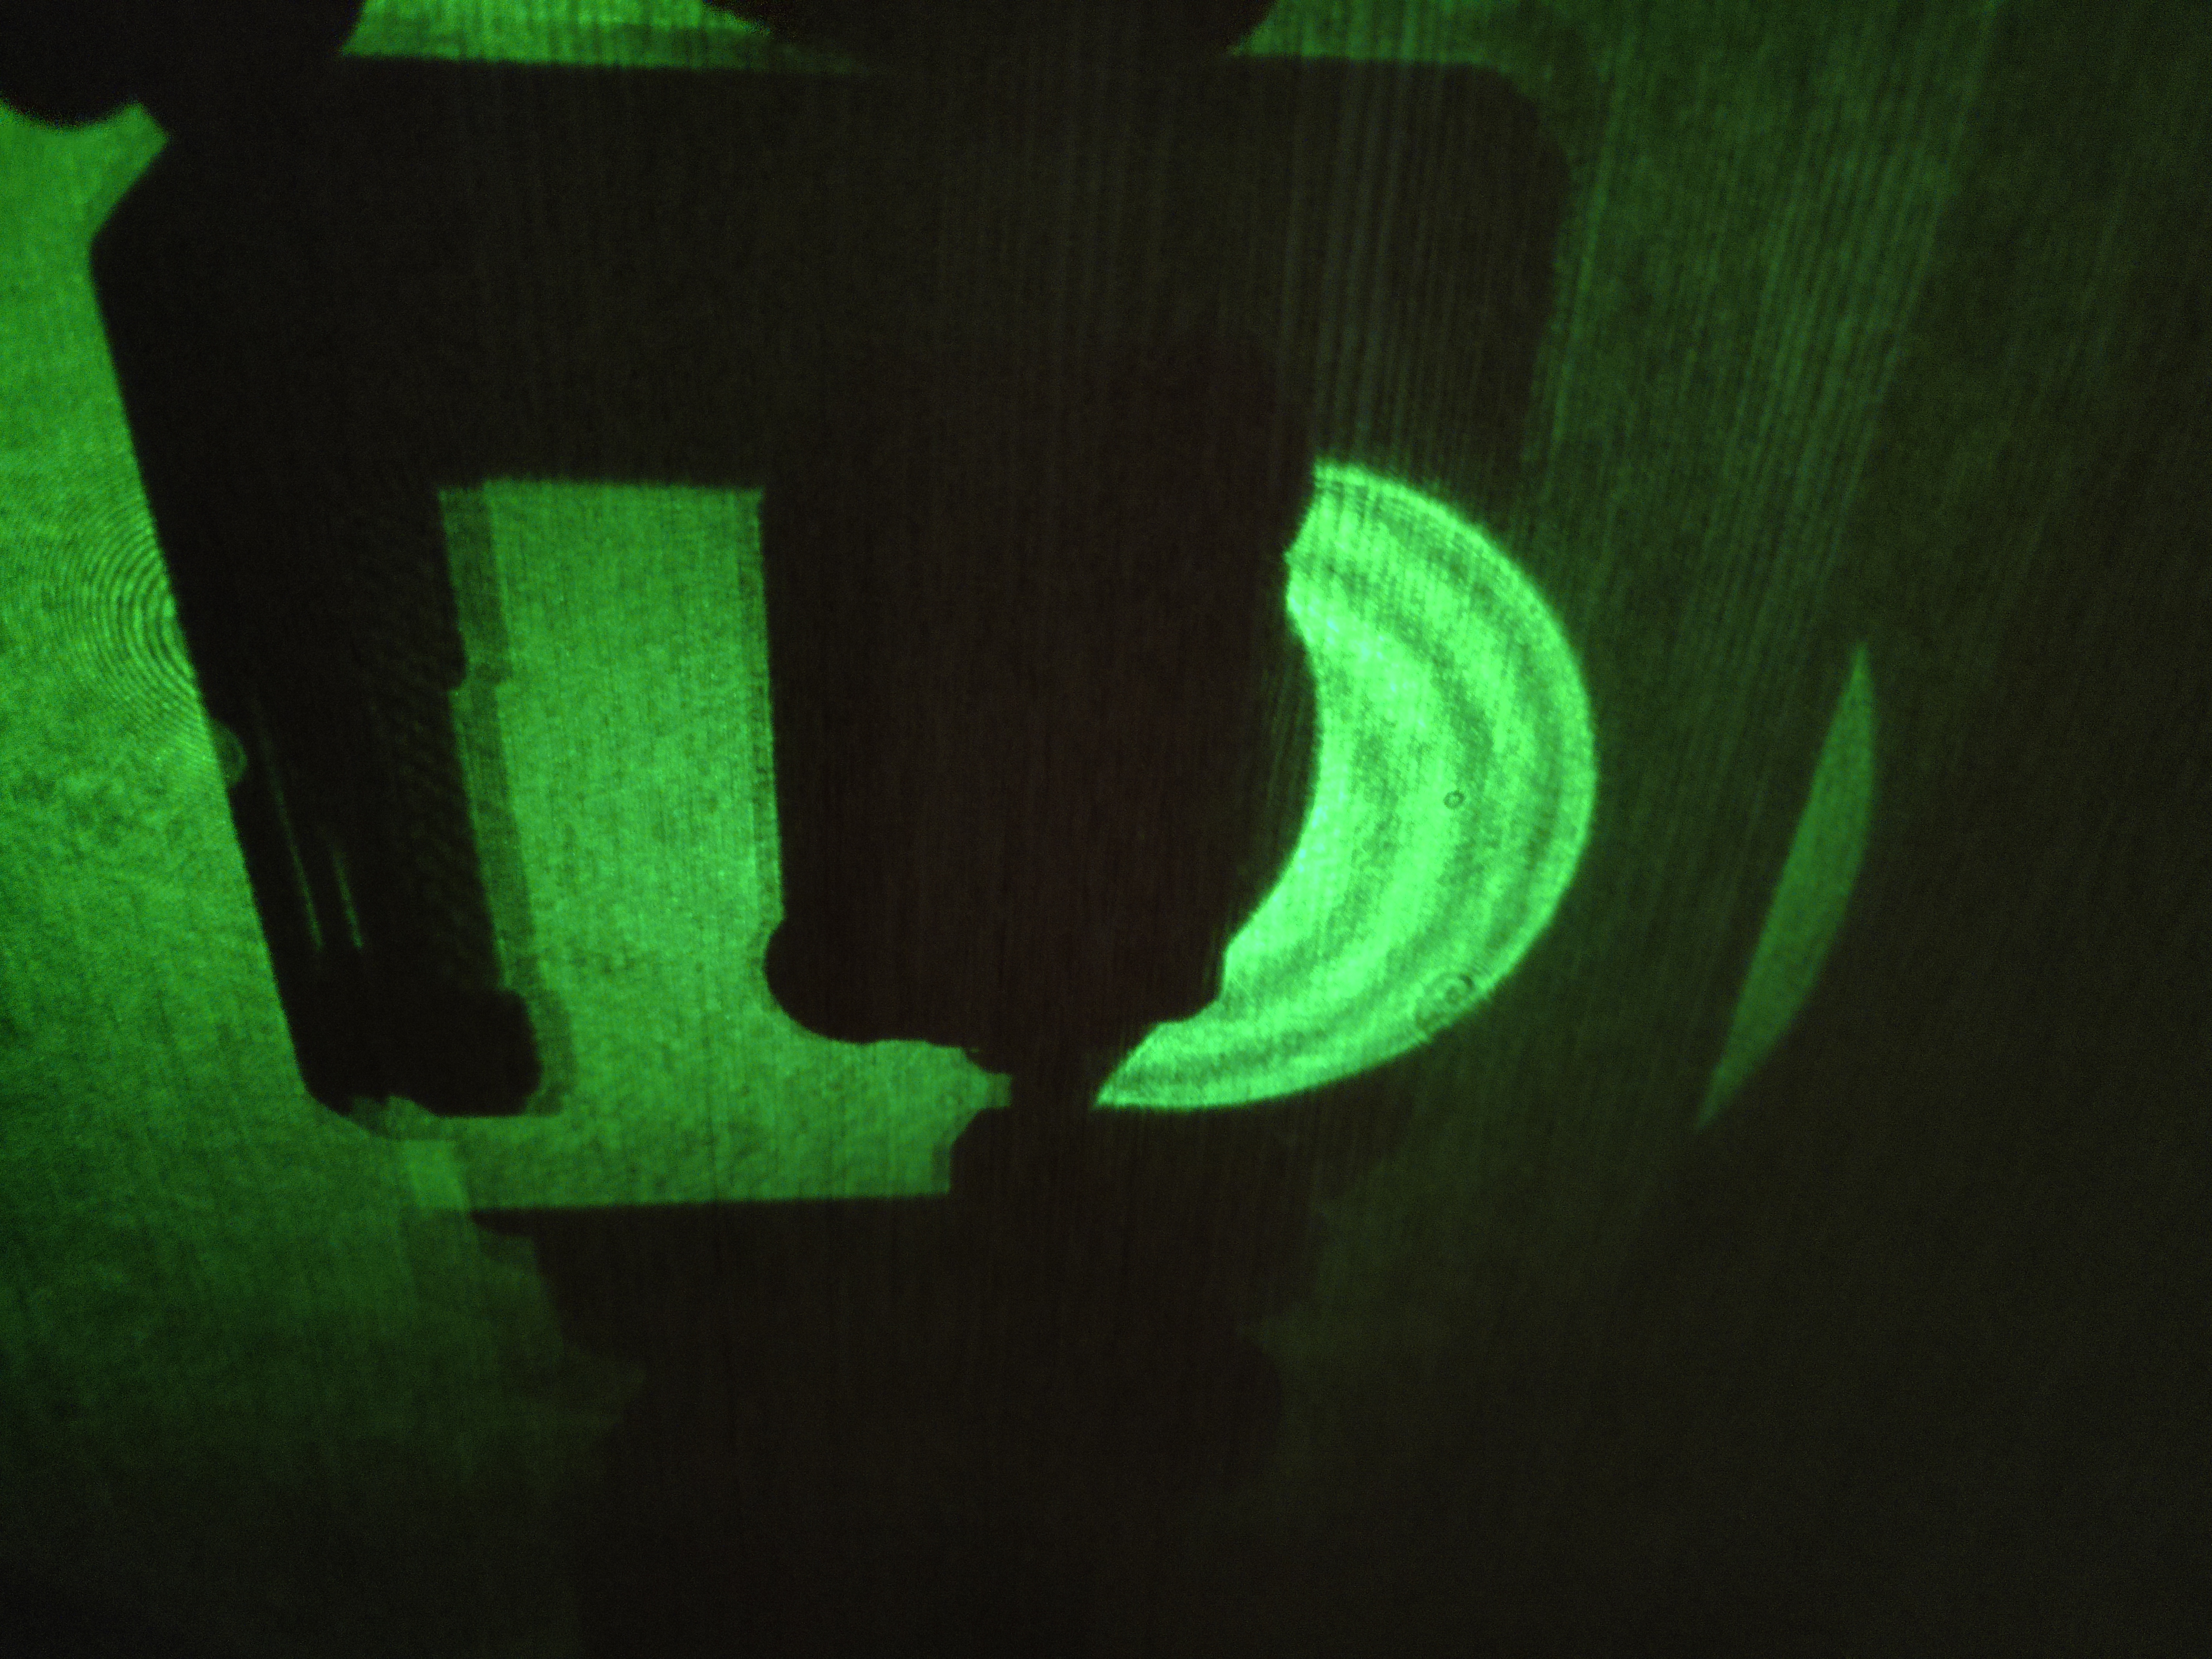
\includegraphics[width=\linewidth]{fig/Sammellinse.png}
        \caption[Strahlengang einer Sammellinse]{Strahlengang zur Abbildung mithilfe einer einzelnen Sammellinse zusammen mit den wichtigsten Parametern. Konstruktion eines Bildes: Parallelstrahl wird zum Brennstrahl (grün) und Brennstrahl zum Parallelstrahl (gelb). Schnittpunkt mit Mittelpunktstrahl (blau) definiert Bildweite $b$ und Bildgröße $B$.}
        \label{fig:sammellinse}
    \end{samepage}
\end{figure}

\paragraph{Methode 3.}
Zuletzt wird zur Bestimmung der Brennweite das sogenannte \textit{Bessel-Verfahren} oder \textit{Bessel'sches Verschiebeverfahren} verwendet. Hierzu wird wieder ein Gegenstand im Versuchsaufbau mit der Linse scharf abgebildet (auf Mattscheibe oder Kamera). Bei festem Abstand $l$ von Gegenstand und Position des scharf abgebildeten Bildes ($l = b + g = \text{const.}$) lässt sich eine zweite Position der Linse finden, für die eine scharfe Abbildung möglich ist ($l = b_1 + g_1 = b_2 + g_2$). Aus dem Gesamtabstand $l$ und den Abstand $w$ zwischen beiden Linsenpositionen lässt sich letztendlich die Brennweite $f$ bestimmen. Dazu gilt folgende Gleichung unter der Annahme dünner Linsen:
%
\begin{equation}
    \label{eq:bessel}
    f = \frac{l^2 - w^2}{4 l}
\end{equation}


\subsection{Das 1-Linsen-Mikroskop nach van Leeuwenhoek}
\label{subsec:1_linsen_mikroskop_Grundlagen}

Antonie van Leeuwenhoek (1632-1723) gilt als einer der ersten erfolgreichen Konstrukteure von einfachen Mikroskopen mit (bis zu seiner Zeit) unerreicht hohen Vergrößerungen und beeindruckender Bildqualität. Durch die hohe Qualität der Linsen und die clevere Konstruktion seiner 1-Linsen-Mikroskope, die teils eher an sehr starke Lupen erinnern, konnte er Auflösungen im Mikrometerbereich erreichen und Mikroorganismen abbilden (und diese dabei auch erstmals nachweisen!). Aufgrund dieser Erfolge wird er auch als Vater der Mikrobakteriologie bzw. Mikrobiologie bezeichnet. Um die genauen Methoden seiner mikroskopischen Messungen ranken sich viele Mythen und Interpretationsversuche, da er die Details bzgl. der Messprozedur sowie der genauen Vorgehensweise zur Herstellung von Linsen, das Kernstück seiner Geräte, stets geheim hielt.
%
\begin{figure}[H]
    \centering
    \begin{samepage}
        \includegraphics[width=\linewidth]{fig/Leeuwenhoek.png}
        \caption[Aufbau eines Van-Leeuwenhoek-Mikroskops]{(a) Bild eines einfachen Mikroskops von van Leeuwenhoek mit Beschreibung der einzelnen Bauteile. (b) Einzelteile des Selbstbau-1-Linsen-Mikroskops angelehnt an van Leeuwenhoek. Auf dem Bild zu sehen sind die 3D-gedruckten Bauteile zur Halterung von Probe, Linsen und Beleuchtung sowie weitere Elemente (Batterie, LED, Schraube, Klammer, Kugellinsen). (c) Fertiggestelltes Selbstbau-1-Linsen-Mikroskop.}
        \label{fig:leeuwenhoek}
    \end{samepage}
\end{figure}
%
Im Folgenden findet sich eine Liste der Bauteile (siehe auch \autoref{fig:leeuwenhoek}):
%
\begin{itemize}
    \item[2] Glaskugeln verschiedenen Durchmessers ($\SI{2,5}{mm}$ und $\SI{6,35}{mm}$) als Linsen mit Brechungsindex $n = \num{1,518}$
    \item[1] Halterung für beide Linsen
    \item[1] Weißlicht-LED als Beleuchtung
    \item[1] Batterie (Knopfzelle CR2032)
    \item[2] Papierklammern (Probenbefestigung)
    \item[1] Trägerplatte zur Befestigung der Probenhalterung
    \item[1] Schraube zur Befestigung des Linsenhalters an der Trägerplatte
\end{itemize}
%
Zur Bestimmung der geforderten Größen, der Lupenvergrößerung $M$ sowie der effektiven Fokuslänge $f$ werden noch die folgenden Gleichungen benötigt:
%
\begin{equation}
    \label{eq:vergroesserung_leeuwenhoek}
    M = \frac{\SI{250}{mm}}{f}
\end{equation}
%
\begin{equation}
    \label{eq:fokuslaenge_leeuwenhoek}
    f = \frac{n \cdot d}{4(n-1)}
\end{equation}
%
Dabei steht $d$ für den Durchmesser der Kugellinse und $n$ bezeichnet die Brechzahl der Linse.


\subsection{Hellfeld-Transmissionsmikroskop}
\label{subsec:hellfeld_transmissionsmikroskop_grundlagen}

Ein konventionelles Mikroskop (griechisch: \textit{mikros} = klein; \textit{skopein} = betrachten) besteht in der Regel aus mindestens zwei Linsen und erlaubt -- wie der Name schon vermuten lässt -- die Betrachtung bzw. Vergrößerung von Objekten, die sich mit dem bloßen Auge eben nicht erkennen/auflösen lassen. Im einfachsten Falle kommen also zwei Linsen zum Einsatz (siehe \autoref{fig:hellfeld_skizze}), wobei eine davon als Objektiv (nahe dem Objekt) und die andere als Okular (nahe dem Auge, lateinisch: \textit{oculus}) fungiert. Das Objektiv erzeugt dabei ein vergrößertes Zwischenbild des Objekts, welches seinerseits durch das Okular weiter vergrößert wird (wie durch eine zusätzliche Lupe). Es ergibt sich eine Gesamtvergrößerung des Objekts durch das System. Fallen die Position des Zwischenbildes und des vorderen Brennpunkts des Okulars zusammen, so entsteht ein Bild im Unendlichen (siehe \autoref{fig:hellfeld_skizze}), welches durch die entspannte Augenlinse auf der Netzhaut zu einem scharfen gesamtvergrößerten Bild wird. Befände sich das Zwischenbild näher am Okular, so entsteht ein virtuelles Zwischenbild, welches für das angespannte Auge in einer effektiven Bezugssehweite von etwa $\SI{25}{cm}$ liegt. Es gibt unzählige Arten von Mikroskopen, die alle Vor- und Nachteile mit sich bringen und die finale Wahl der Methode hängt meist vom abzubildenden System ab.
%
\begin{figure}[H]
    \centering
    \begin{samepage}
        \includegraphics[width=\linewidth]{fig/Hellfeld.png}
        \caption[Aufbau eines Hellfeld-Transmissionsmikroskops]{Schematischer Aufbau und Bildkonstruktion eines Mikroskops bestehend aus Gegenstand/Objekt, Objektivlinse und Okularlinse. Die entsprechenden Brennweiten und weitere Parameter sind im Bild vermerkt. Das Okular ist hier so platziert, dass dessen Brennpunkt und die Position des Zwischenbildes (ZB) zusammenfallen. Dadurch entstünde ein Bild im Unendlichen. Mithilfe der (entspannten auf Unendlich akkommodierten) Augenlinse oder eben einer Kameralinse entsteht letztendlich ein scharfes, gesamtvergrößertes Bild (hier nicht eingezeichnet). Auch die Beleuchtung des Gegenstandes ist nicht eingezeichnet. Den Abstand zwischen hinterem Brennpunkt des Objektivs und vorderem Brennpunkt des Okulars nennt man optische Tubuslänge $t_o$.}
        \label{fig:hellfeld_skizze}
    \end{samepage}
\end{figure}
%
% Die Bestimmung der Gesamtvergrößerung $G$ erfolgt über die Pixelgröße $P_A$ und die Pixelanzahl $P_n$ sowie das Auflösungsvermögen nach \autoref{eq:gesamtvergroesserung_hellfeld}.
% %
% \begin{equation}
%     \label{eq:gesamtvergroesserung_hellfeld}
%     G = \frac{P_A P_n}{N}
% \end{equation}

Fallen Zwischenbild und vorderer Brennpunkt des Okulars zusammen, so ist die Vergrößerung $V_{\text{MIK}}$ des Systems definiert als das Produkt des Objektiv-Abbildungsmaßstabs $A_{\text{obj}}$ und der Okularvergrößerung $V_{\text{oku}}$.
%
\begin{equation}
    \label{eq:objektivabbildungsmaszstab}
    A_{\text{obj}} = -\frac{t_o}{f_{\text{obj}}}
\end{equation}
\begin{equation}
    \label{eq:okularvergroeszerung}
    V_{\text{oku}} = \frac{\SI{25}{cm}}{f_{\text{oku}}}
\end{equation}
\begin{equation}
    \label{eq:gesamtvergroesserung}
    V_{\text{MIK}} = A_{\text{obj}} \cdot V_{\text{oku}}
\end{equation}

Eine wichtige Größe bei Mikroskopen ist deren \textit{Auflösungsvermögen} $x_\text{min}$. Es beschreibt den kleinsten Abstand, bei welchem zwei Objekte noch getrennt voneinander wahrgenommen werden können, dies ist das Ergebnis der Abbe'schen Abbildungstheorie.

Im zentralen Bereich der Probe befinden sich verschiedene Gruppen ($G$), welche jeweils aus mehreren Elementen ($E$) aufgebaut sind. Jede Gruppe (Nummerierung jeweils oben) besteht aus sechs Elementen (Nummerierung seitlich). Jedes Element besteht dabei aus drei horizontalen und drei vertikalen Balken. Je höher die Nummerierung, desto kleiner die Balken.

In diesem Experiment lässt sich das Auflösungsvermögen über die Balken- und Gruppennummer der Probe berechnen. Hierbei kann die \textit{Ortsfrequenz} $f_r$ folgendermaßen bestimmt werden:
%
\begin{equation}
    \label{eq:ortsfrequenz}
    f_r = 2^{G+\frac{E-1}{6}}
\end{equation}
%
Die Einheit der Ortsfrequenz ist hierbei die Anzahl der Linienpaare pro Millimeter (\si{LP\per\milli\meter}). $G$ beschreibt die Gruppenummer und $E$ die Elementnummer. Das Auflösungsvermögen lässt sich schließlich über den Kehrwert der Ortsfrequenz berechnen:
%
\begin{equation}
    \label{eq:aufloesungsvermoegen}
    x_\text{min} = \frac{1}{f_r}
\end{equation}


\subsection{Dunkelfeldmikroskop}
\label{subsec:dunkelfeldmikroskop_grundlagen}

Wie im vorherigen Abschnitt bereits beschrieben spielt die Art der Beleuchtung eine große Rolle. Dabei sind die Wellenlänge oder auch die spektrale Breite, die Homogenität und der Winkelbereich der Beleuchtung von großer Wichtigkeit. Nun sollen diese Aspekte erneut in Bezug auf Dunkelfeld-Beleuchtung bzw. -Mikroskope aufgegriffen werden. Erste Ansätze in Richtung dieser Methode werden van Leeuwenhoek, Hooke und Huygens zugeschrieben. Im Vergleich zu einem Hellfeld-Mikroskop, bei dem die Strukturen einer Probe vor einem hellen Hintergrund erscheinen und sich vor allem durch Absorption und durch Streuung verloren gegangenes Licht von diesem abheben, wird beim Dunkelfeld-Prinzip nur dort Licht aufgesammelt, wo die Probe Licht in eine Aufsammeloptik (Linse/Objektiv) hineinstreut. Bereiche, in denen es zu keiner Streuung kommt, erscheinen im Bild also schwarz. Dies kann bei wenig absorbierenden Proben von großem Vorteil in Sachen Bildkontrast sein. In \autoref{fig:dunkelfeld_skizze} ist ein Vergleich aus Hellfeld- und Dunkelfeld-Beleuchtung gezeigt. Man sieht deutlich, wie im Falle einer Hellfeld-Beleuchtung (\autoref{fig:dunkelfeld_skizze}, links) die Probe ausgeleuchtet und das transmittierte Licht gemessen wird. Wird Licht vom Objekt reflektiert, absorbiert oder so gestreut, dass es die Aufsammeloptik nicht erreicht, so wird dort im Bild die Intensität geringer sein, als an Orten, an denen das Licht nahezu ungehindert die Probe durchlaufen konnte. Das Bild erscheint also als dunklerer Bereich auf hellem Hintergrund. Fand wenig Absorption, Streuung oder Reflexion statt, ist der Kontrast (Helligkeitsunterschied) sehr gering. Wenn hingegen \autoref{fig:dunkelfeld_skizze} (rechts) betrachtet wird, so sieht man deutlich, dass die Dunkelfeld-Beleuchtung zu einer vollkommen anderen Bilderzeugung führt, deren Kontrastmechanismus auch stark von der Hellfeld-Methode abweicht. Das Licht, welches die Probe nahezu ungehindert durchläuft, liegt außerhalb des Winkelbereichs der Aufsammeloptik (streifender Einfall der Beleuchtung). Entsprechende Bereiche werden im Bild als Hintergrund also schwarz/dunkel erscheinen. Werden aber Teile des Lichts in Bereiche des Objekts gestreut und dabei so umgelenkt, dass sie aufgesammelt werden können, so zeichnen sich diese Bereiche also hell ab. Es entsteht ein entsprechender Kontrast. Die Absorption spielt hierbei eine untergeordnete Rolle.
%
\begin{figure}[H]
    \centering
    \begin{samepage}
        \includegraphics[width=\linewidth]{fig/Hell_vs_Dunkelfeld.png}
        \caption[Aufbau eines Dunkelfeldmikroskop]{Vergleich Hellfeld- (links) und Dunkelfeld-Methode (rechts). Beleuchtung/Licht (rot) von unten kommend. Zentralblende (rechts; schwarz) lässt nur Randstrahlen passieren.}
        \label{fig:dunkelfeld_skizze}
    \end{samepage}
\end{figure}


\subsection{Unsicherheitsanalyse}
\label{subsec:unsicherheitsanalyse}

Die explizit angegebenen Unsicherheiten der ermittelten Messgrößen basieren auf Berechnungen durch die Unsicherheitsangabe nach den Datenblättern der verwendeten Messgeräte. Diese sind in \autoref{tab:geraeteliste} vermerkt beziehungsweise referenziert.

Die Fehlerfortpflanzung der berechneten Werte basiert auf der Größtunsicherheitsmethode nach Gauß. Um diese Berechnungen zeiteffizient durchführen zu können, wird für jeden Unterpunkt der Laborübung ein Skript in \verb!Python! implementiert. Kernstück dessen ist das package \verb!uncertainties! \cite{ref:uncertainties}, das intern die Fehlerfortpflanzung berechnet. Gerundet wird nach den Angaben des Skriptums der Lehrveranstaltung \enquote{Einführung in die physikalischen Messmethoden} \cite{ref:messmethoden}.



\section{Versuchsanordnung}
\label{sec:versuchsanordnung}

\subsection{Brennweite der Sammellinse}
\label{subsec:versuchsanordnung_sammellinse}

Die Bestimmung der Brennweite wird, wie in \autoref{sec:aufgabenstellung} angeführt, mittels dreier verschiedener Ansätze vorgenommen.

Der Aufbau ist für die unterschiedlichen Verfahren großteils gleich, Abweichungen davon werden in \autoref{sec:versuchsdurchfuehrung_messergebnisse} beschrieben. Die Bauteile werden allesamt auf einer Aluminiumschiene fixiert, wodurch eine möglichst lineare Anordnung und dadurch auch ein möglichst paralleler Strahlengang erreicht werden kann.
Der grundsätzliche Aufbau ist \autoref{fig:versuchsaufbau_sammellinse} zu entnehmen.
%
\begin{figure}[H]
    \centering
    \begin{samepage}
        \includegraphics[width=\linewidth]{fig/versuch1.jpeg}
        \caption[Aufbau Brennweite einer Sammellinse bestimmen]{Aufbau zur Bestimmung der Brennweite einer Sammellinse. Komponenten von links nach rechts: Lampe, Diffusor, Probenhalter inkl. Probe, plankonvexe Linse (planare Seite objektseitig), Kamera}
        \label{fig:versuchsaufbau_sammellinse}
    \end{samepage}
\end{figure}


\subsection{Van-Leeuwenhoek-Mikroskop}
\label{subsec:versuchsanordnung_vanleeuwenhoek}

Das Van-Leeuwenhoek-Mikroskop wird nach den Beschreibungen in \cite{ref:angabe} zusammengebaut. Dazu wird die Knopfbatterie in das dafür vorgesehene Fach gegeben und die beiden LED-Kontakte mit der richtigen Polarität zwischen Plastik und Zelle eingeklemmt. Die LED dient der Beleuchtung der Proben. Nun bringt man mittels der Schraube noch den Arm mit den beiden Linsen an und der Aufbau ist vollständig.


\subsection{Hellfeld-Transmissionsmikroskop}
\label{subsec:versuchsanordnung_hellfeld}

Der Versuchsaufbau aus \autoref{subsec:versuchsanordnung_sammellinse} wird übernommen und anschließend wie folgt geändert: Zuerst wird die plankonvexe Linse gegen eine Linse mit $f = \SI{35}{mm}$ (objektivseitig) ausgetauscht. Diese Linse wird in einem Abstand $g_{\text{obj}}$ von $\SI{44(1)}{mm}$ eingesetzt. Das Okular mit Brennweite $f = \SI{50}{mm}$ wird im Abstand von $\SI{210(6)}{mm}$ von der Probe eingebaut. Die Kamera wird mit angeschraubter Linse mit $f = \SI{150}{mm}$ im Abstand von $\SI{200(5)}{mm}$ angebracht. % info den Abstand haben wir zuerst glaub ich ned gemessen, falls doch bitte korrigieren.
Der Aufbau wird nochmals in \autoref{fig:versuchsaufbau_hellfeld} verdeutlicht.
%
\begin{figure}[H]
    \centering
    \begin{samepage}
        \includegraphics[width=\linewidth]{fig/Hellfeld_.jpeg}
        \caption{Aufbau eines Hellfeld-Transmissionsmikroskops}
        \label{fig:versuchsaufbau_hellfeld}
    \end{samepage}
\end{figure}


\subsection{Dunkelfeldmikroskop}
\label{subsec:versuchsanordnung_dunkelfeld}

Für den Dunkelfeldaufbau wird der Diffusor aus dem Strahlengang genommen und ein spezielles Objektiv eingesetzt, dieses hat bereits eine Blende integriert, welche nur einen peripheren Ring zur Beleuchtung der Probe offenlässt. Nach der Probe wird anstelle der in den vorherigen Versuchen benutzten Linsen eine achromatische Linse mit $f = \SI{25}{mm}$ eingebracht und die Kamera abermals ohne angeschraubt Linse befestigt. Die achromatische Linse verfügt zudem noch über eine Irisblende, um nur das Streulicht der Probe, nicht aber das direkte Licht in die Kamera zu lassen. Der Aufbau wird in \autoref{fig:versuchsaufbau_dunkelfeld} dargestellt.
%
\begin{figure}[H]
    \centering
    \begin{samepage}
        \includegraphics[width=\linewidth]{fig/Dunkelfeld.jpeg}
        \caption{Aufbau eines Dunkelfeldmikroskops}
        \label{fig:versuchsaufbau_dunkelfeld}
    \end{samepage}
\end{figure}



\section{Geräteliste}
\label{sec:geraeteliste}

\begin{table}[H]
    \centering
    \begin{samepage}  % caption and table on same page
        \caption[Geräteliste]{Verwendete Geräte und wichtige Materialien}  % optional argument for List of Tables, mandatory argument for caption
        \label{tab:geraeteliste}
        \begin{tblrx}{colspec={QQQQQ}, row{1}={guard}}
            Gerät                     & Hersteller & Modell & Inventar-Nr.   & Anmerkung                                                     \\
            QTH10/M                   & THORLABS   & -                       & -              & inkl. Infrarot Filter                                         \\
            LED $2\times$             & THORLABS   & -                       & -              & rot \& blau                                                   \\
            Diffusor                  & -          & -                       & -              & -                                                             \\
            Probenhalter XYF1         & THORLABS   & -                       & -              & -                                                             \\
            Probe                     & THORLABS   & -                       & -              & -                                                             \\
            Plankonvexe Sammellinsen  & -          & -                       & -              & unbekannte Brennweite                                         \\
            Optischer Tisch           & -          & -                       & -              & inkl. Befestigungsschienen                                    \\
            Van Leeuwenhoek Mikroskop & 3D-Drucker & -                       & -              & inkl. Schraube, LED \& Batterie                               \\
            Kamerasensor              & CS165MU/M  & -                       & -              & $\SI{1,6}{\mega\px}$ -- Pixelgröße: $\SI{3,45}{\micro\meter}$ \\
            Kamerasoftware            & THORLABS   & ThorCam\texttrademark{} & -              & $\SI{1,6}{\mega\px}$ -- Pixelgröße: $\SI{3,45}{\micro\meter}$ \\
            Kameraobjektiv            & -          & -                       & -              & $f=\SI{150}{mm}$                                              \\
            Objektiv                  & -          & -                       & -              & $f=\SI{35}{mm}$                                               \\
            Okular                    & -          & -                       & -              & $f=\SI{50}{mm}$                                               \\
            Mikroskopobjektiv         & Nikon      & -                       & -              & Vergrößerung: $10 \times$                                     \\
            Achromatische Linse       & -          & -                       & -              & $f=\SI{25}{mm}$, inkl. Irisblende                             \\
        \end{tblrx}
    \end{samepage}
\end{table}



\section{Versuchsdurchführung und Messergebnisse}
\label{sec:versuchsdurchfuehrung_messergebnisse}

\subsection{Brennweite einer Sammellinse}
\label{subsec:durchfuehrung_brennweite_sammellinse}

Der Aufbau wird, wie auf \autoref{fig:versuchsaufbau_sammellinse} gezeigt, hergestellt.


\paragraph{Lupeneffekt.}
Um zuallererst die Brennweite mittels Lupeneffekt abzuschätzen, gilt die Annahme, dass das Bild im Unendlichen entsteht. Als beweglicher Schirm für das reelle Bild fungiert ein weißes Blatt Papier. In einem Zusammenspiel aus Veränderung der Linsenposition relativ zur optischen Probe und dem Schirm in Form des weißen Blatt Papiers wird eine Anordnung gefunden, bei welcher das Bild in großer Entfernung von der Linse scharf wirkt. Unter der Annahme, dass die Strahlen parallel verlaufen, ist dieses Bild auch im Unendlichen noch scharf. Bei dieser Konfiguration wird die Gegenstandsweite $g$ -- der Abstand von optischer Probe zur Linse -- vermessen und mit
\[g=\SI{20(2)}{mm}\]
beziffert.


\paragraph{Abbildungsgleichung.}
Als Nächstes wird die Brennweite der Linse über die Abbildungsgleichung (\autoref{eq:linsengleichung}) bestimmt. Hierzu wird der Abstand des Gegenstands, also der Probe, sowie der Abstand des entstehenden Bilds zur Linse gemessen. Diese Messung wird je zweimal wiederholt, allerdings mit unterschiedlichen Positionen der Linse, sodass zwei unabhängige Kombinationen von $g$ und $b$ ergeben. Die Messergebnisse finden sich in \autoref{tab:messergebnisse_brennweite_gleichung}.
%
\begin{table}[H]
    \centering
    \begin{samepage}
        \caption[Messergebnisse Brennweite Abbildungsgleichung]{Messergebnisse des Teilversuchs zur Bestimmung der Brennweite einer Linse mittels Abbildungsgleichung. $g$ bezeichnet die Gegenstandsweite, $b$ die Bildweite, $i$ den Laufindex der Position der Linse. Unsicherheiten: $\Delta g$, $\Delta b$.}
        \label{tab:messergebnisse_brennweite_gleichung}
        \begin{tblr}{colspec={QS[table-format=3]S[table-format=1]S[table-format=2]S[table-format=1]}, row{1}={guard}}
            $i$ / 1 & $g$ / \si{mm} & $\Delta g$ / \si{mm} & $b$ / \si{mm} & $\Delta b$ / \si{mm} \\
            1       & 126           & 3                    & 35            & 2                    \\
            2       & 44            & 2                    & 54            & 2                    \\
        \end{tblr}
    \end{samepage}
\end{table}


\paragraph{Bessel-Verfahren.}
Zuletzt wird die Brennweite der Linse noch über das Bessel-Verfahren, wie in \autoref{subsec:abbildung_sammellinse_Grundlagen} beschrieben, vermessen. Es wird eine beliebige Position der Linse gewählt und sowohl die Gegenstandsweite $g$ als auch die Bildweite $b$ vermessen. Die Summe dieser beiden ergibt die Gesamtlänge $l$. Danach wird eine neue Position der Linse gewählt, sodass sich die Gesamtlänge nicht verändert. Die gemessenen Bildweiten und Gegenstandsweiten befinden sich in \autoref{tab:messergebnisse_brennweite_bessel}.
%
\begin{table}[H]
    \centering
    \begin{samepage}
        \caption[Messergebnisse Brennweite Bessel]{Messergebnisse des Teilversuchs zur Bestimmung der Brennweite einer Linse mittels Bessel-Verfahren. $g$ bezeichnet die Gegenstandsweite, $b$ die Bildweite, $i$ den Laufindex der Position der Linse. Unsicherheiten: $\Delta g$, $\Delta b$.}
        \label{tab:messergebnisse_brennweite_bessel}
        \begin{tblr}{colspec={QS[table-format=3]S[table-format=1]S[table-format=3]S[table-format=1]}, row{1}={guard}}
            $i$ / 1 & $g$ / \si{mm} & $\Delta g$ / \si{mm} & $b$ / \si{mm} & $\Delta b$ / \si{mm} \\
            1       & 23            & 2                    & 125           & 3                    \\
            2       & 112           & 3                    & 36            & 3                    \\
        \end{tblr}
    \end{samepage}
\end{table}


\subsection{Van-Leeuwenhoek-Mikroskop}
\label{subsec:durchfuehrung_vanleeuwenhoek}

Der Aufbau wird, wie in \autoref{subsec:versuchsanordnung_vanleeuwenhoek} beschrieben, hergestellt. Anschließend werden als zu untersuchende Proben eine Kugelschreiberspitze und ein Blatt Papier herangezogen. Durch die Kugellinse konnten dann tatsächlich vergrößerte Bilder der genannten Proben betrachtet werden, obgleich es nicht ganz einfach war, die richtige Position zu finden, bei der man dann tatsächlich ein Bild erkennen konnte. Mithilfe der Makro-Kamera des Smartphones eines Experimentierenden konnten sogar digitale Abbildungen der vergrößerten Bilder aufgenommen werden. Dies ist jedoch nur mit der größeren Kugellinse möglich, das Bild der kleineren lässt sich mit der Kamera nicht auflösen. Die Abbildungen der größeren Linse finden sich in den Abbildungen \ref{fig:vanleeuwenhoek_kugelschreiber} und \ref{fig:vanleeuwenhoek_papier}.
%
\setcapindent{0pt}
\begin{figure}[H]
    \centering
    \begin{minipage}[b]{0.475\linewidth}
        \centering
        \includegraphics[width=\linewidth]{fig/Kulli.jpeg}
        \caption[Kugelschreiberspitze Van-Leeuwenhoek]{Durch die größere Linse des Van-Leeuwenhoek-Mikroskops vergrößerte Kugelschreiberspitze}
        \label{fig:vanleeuwenhoek_kugelschreiber}
    \end{minipage}%
    \hspace*{\fill}
    \begin{minipage}[t]{0.475\linewidth}
        \centering
        \includegraphics[width=0.75\linewidth]{fig/papier_gross.jpeg}
        \caption[Blatt Papier Van-Leeuwenhoek]{Durch die größere Linse des Van-Leeuwenhoek-Mikroskops vergrößertes Blatt Papier}
        \label{fig:vanleeuwenhoek_papier}
    \end{minipage}
\end{figure}
\setcaphanging
%
Betrachtet man weiters den Unterschied der beiden am Mikroskoparm angebrachten Linsen so wird ersichtlich, dass die Kugellinse mit größerem Durchmesser eine stärkere Vergrößerung als die mit kleinerem Durchmesser aufweist. Gemein ist beiden Linsen jedoch eine deutlich erkennbare Bildfeldwölbung.


\subsection{Hellfeld-Transmissionsmikroskop}
\label{subsec:durchfuehrung_hellfeld}

Der Aufbau wird, wie in \autoref{subsec:versuchsanordnung_hellfeld} beschrieben, hergestellt.

Anschließend werden relevante Abstände der Aufbaut vermessen: Der Abstand der Objektivlinse (mit Brennweite $f_{\text{obj}}=\SI{35.0(4)}{mm}$) zur optischen Probe wird vermessen und mit $g_{\text{obj}}=\SI{44(1)}{mm}$ beziffert. Der Abstand zwischen Objektiv- und Okularlinse beträgt $d_{\text{obj-oku}}=\SI{170(5)}{mm}$. Die Brennweite der verwendeten Okularlinse beträgt $f_{\text{oku}}=\SI{50.0(4)}{mm}$ und deren Abstand zur Probe beträgt $d_{\text{prob-oku}}=\SI{210(5)}{mm}$.

Als Nächstes wird die Auswirkung von Aberationseffekten auf das Bild der Linse untersucht.

\paragraph{Objektivlinsenorientierung und sphärische Aberration.}
Nachdem bereits ein scharfes Bild zustande gebracht worden ist, wird dieses mittels Kamera aufgenommen und abgespeichert. Es gilt als Referenzbild im Ausgangszustand der Anordnung. Dieses Bild findet sich in \autoref{fig:hellfeld_orientierung_sphaerische_ref}.
%
\begin{figure}[H]
    \centering
    \begin{samepage}
        \includegraphics[width=0.475\linewidth]{fig/Versuch3/hellfeld_3.1_vorher.jpg}
        \caption[Hellfeld Orientierung und sphärische Aberration]{Referenzbild des Teilversuchs zur Untersuchung der Auswirkung der Objektivlinsenorientierung und der sphärischen Aberration auf das entstehende reelle Bild.}
        \label{fig:hellfeld_orientierung_sphaerische_ref}
    \end{samepage}
\end{figure}
%
Anschließend wird die Objektiv-Linse mitsamt Halterung um \SI{180}{\degree} gedreht. Nun weist die gekrümmte Seite der Linse in Richtung Probe. Erneut wird ein Bild aufgenommen, dieses ist jedoch nicht scharf. Mit dem Feinregler wird die Position der Probe justiert, sodass wieder ein scharfes Bild entsteht. Das scharfe sowie unscharfe Bild sind nebeneinander in den Abbildungen \ref{fig:hellfeld_orientierung_sphaerische_gedreht_unscharf} und \ref{fig:hellfeld_orientierung_sphaerische_gedreht_scharf} dargestellt.
%
\setcapindent{0pt}
\begin{figure}[H]
    \centering
    \begin{minipage}[t]{0.475\linewidth}
        \centering
        \includegraphics[width=\linewidth]{fig/Versuch3/hellfeld_3.1_nachher.jpg}
        \caption[Hellfeld Orientierung und sphärische Aberration gedreht unscharf]{Unscharfe Abbildung bei um \SI{180}{\degree} gedrehter Objektiv-Linse (konvexe Seite zeigt zur Probe)}
        \label{fig:hellfeld_orientierung_sphaerische_gedreht_unscharf}
    \end{minipage}%
    \hspace*{\fill}
    \begin{minipage}[t]{0.475\linewidth}
        \centering
        \includegraphics[width=\linewidth]{fig/Versuch3/hellfeld_3.1_vorher.jpg}
        \caption[Hellfeld Orientierung und sphärische Aberration gedreht scharf]{Scharfe Abbildung bei um \SI{180}{\degree} gedrehter Objektiv-Linse (konvexe Seite zeigt zur Probe)}
        \label{fig:hellfeld_orientierung_sphaerische_gedreht_scharf}
    \end{minipage}
\end{figure}
\setcaphanging

\paragraph{Kohärenz.}
Als Nächstes wird die Auswirkung der Kohärenz der Beleuchtung auf die Bildgebung untersucht. Hierzu wird der Diffusor zwischen Lichtquelle und Probe aus dem Aufbau entfernt. Die Position der restlichen Komponenten bleiben unverändert. Es ergibt sich abermals ein unscharfes Bild, welches diesmal jedoch nicht scharfgestellt werden konnte. Dieses Bild befindet sich auf \autoref{fig:hellfeld_ohne_diffusor}.
%
\begin{figure}[H]
    \centering
    \begin{samepage}
        \includegraphics[width=0.475\linewidth]{fig/Versuch3/hellfeld_3.2_ohne_diffusor.jpg}
        \caption[Hellfeld Kohärenz]{Bildgebung nach Entfernung des Diffusors aus dem Aufbau}
        \label{fig:hellfeld_ohne_diffusor}
    \end{samepage}
\end{figure}

\paragraph{Wellenlängenabhängigkeit und chromatische Aberration.}
Zu guter Letzt wird die Wellenlängenabhängigkeit des Bilds untersucht. Hierzu wird die Halogenlampe, die bis eben als Lichtquelle gedient hat, durch eine blaue LED ersetzt. Diese wird über einen USB-Port, welcher mit dem PC verbunden wird, mit Strom versorgt. Es wird wieder ein (unscharfes) Bild aufgenommen (\autoref{fig:Hellfeld_3_3_blau_unscharf}) und scharfgestellt (\autoref{fig:Hellfeld_3_3_blau_scharf}). Anschließend wird die blaue LED durch eine rote LED ersetzt. Auch hier wird wieder ein Bild aufgenommen und scharfgestellt. Die Bilder sind in \autoref{fig:Hellfeld_3_3_rot_unscharf} und \autoref{fig:Hellfeld_3_3_rot_scharf} dargestellt. Für beide LED-Lichtquellen wird darüber hinaus notiert, um welche Distanz die Probe mittels Mikrometerschraube verschoben werden musste, um ein scharfes Bild zu erhalten, relativ zum von derselben Position ausgehenden unscharfen Bild. Für die blaue LED ergibt sich eine Verschiebung von $d_{\text{blau}}=\SI{1.85(5)}{mm}$ und für die rote LED von $d_{\text{rot}}=\SI{1.78(5)}{mm}$.
%
\setcapindent{0pt}
\begin{figure}[H]
    \centering
    \begin{minipage}[t]{0.475\linewidth}
        \centering
        \includegraphics[width=\linewidth]{fig/Versuch3/hellfeld_3.3_blau_unscharf.jpg}
        \caption[Hellfeld LED blau unscharf]{Unscharfes Bild bei Beleuchtung mit blauer LED}
        \label{fig:Hellfeld_3_3_blau_unscharf}
        \includegraphics[width=\linewidth]{fig/Versuch3/hellfeld_3.3_blau_scharf.jpg}
        \caption[Hellfeld LED blau scharf]{Scharfes Bild bei Beleuchtung mit blauer LED}
        \label{fig:Hellfeld_3_3_blau_scharf}
    \end{minipage}%
    \hspace*{\fill}
    \begin{minipage}[t]{0.475\linewidth}
        \centering
        \includegraphics[width=\linewidth]{fig/Versuch3/hellfeld_3.3_rot_unscharf.jpg}
        \caption[Hellfeld LED rot unscharf]{Unscharfes Bild bei Beleuchtung mit roter LED}
        \label{fig:Hellfeld_3_3_rot_unscharf}
        \includegraphics[width=\linewidth]{fig/Versuch3/hellfeld_3.3_rot_scharf.jpg}
        \caption[Hellfeld LED rot scharf]{Scharfes Bild bei Beleuchtung mit roter LED}
        \label{fig:Hellfeld_3_3_rot_scharf}
    \end{minipage}
\end{figure}
\setcaphanging

Als Abschluss wird noch die Gesamtvergrößerung und das Auflösungsvermögen des vorliegenden Aufbaus untersucht.

\paragraph{Gesamtvergrößerung.}
Für die experimentelle Auswertung der Gesamtvergrößerung wird zuerst ein (unvergrößertes) Referenzbild mit Abbildungsmaßstab $A=1$ aufgenommen. Dazu wird die Linse aus dem Strahlengang entfernt, der Aufbau so konfiguriert, dass $b=g=2f$ gilt und der Abstand zweier charakteristischer Punkte in \si{\px} mit dem virtuellen Lineal der am PC laufenden Software \textit{ThorCam\texttrademark{}} aus dem aufgenommenen Bild ausgemessen. Danach wird die Linse wieder eingesetzt und es entsteht ein reelles vergrößertes \emph{verkehrtes} Bild. Derselbe Abstand wird gemessen. Die beiden Bilder und die darin eingetragenen Abstände befinden sich auf den Abbildungen \ref{fig:hellfeld_gesamtvergroeszerung_referenz} und \ref{fig:hellfeld_gesamtvergroeszerung_vergroeszert}.
%
\setcapindent{0pt}
\begin{figure}[H]
    \centering
    \begin{minipage}[t]{0.475\linewidth}
        \centering
        \includegraphics[width=\linewidth]{fig/Versuch3/hellfeld_4.1_referenz.jpg}
        \caption[Hellfeld Gesamtvergrößerung Referenz]{Referenzbild zur Bestimmung der Gesamtvergrößerung. Der Abstand der beiden Eckpunkte der Quadrate ist mittels Software ausgemessen und auf dem Bild eingetragen.}
        \label{fig:hellfeld_gesamtvergroeszerung_referenz}
    \end{minipage}%
    \hspace*{\fill}
    \begin{minipage}[t]{0.475\linewidth}
        \centering
        \includegraphics[width=\linewidth]{fig/Versuch3/hellfeld_4.1_vergroeszert.jpg}
        \caption[Hellfeld Gesamtvergrößerung vergrößert]{Vergrößertes \emph{verkehrtes} Bild zur Bestimmung der Gesamtvergrößerung. Der Abstand der beiden Eckpunkte der Quadrate ist mittels Software ausgemessen und auf dem Bild eingetragen.}
        \label{fig:hellfeld_gesamtvergroeszerung_vergroeszert}
    \end{minipage}
\end{figure}
\setcaphanging
%
Die in den Abbildungen eingetragenen Abstände sind demnach $d_\text{unvergrößert}=\SI{128(7)}{\px}$ und $d_\text{vergrößert}=\SI{84(5)e1}{\px}$. Dabei wird eine Unsicherheit von \SI{5}{\percent} angenommen, die durch das sensible Auswählen der Eckpunkte begründet wird.

\paragraph{Auflösungsvermögen.}
Als Abschluss zum Teilversuch \textit{Hellfeldmikroskop} wird noch das Auflösungsvermögen $x_\text{min}$, das nach \autoref{eq:aufloesungsvermoegen} gegeben ist, bestimmt. Hierzu wird jener Bereich des Probenbilds gesucht, der gerade noch scharf aufgelöst werden kann. Das dafür zur Rate gezogene Bild ist \autoref{fig:hellfeld_aufloesungsvermoegen}.
%
\begin{figure}[H]
    \centering
    \begin{samepage}
        \includegraphics[width=0.475\linewidth]{fig/Versuch3/hellfeld_4.2_aufloesungsvermoegen.jpg}
        \caption[Hellfeld Auflösungsvermögen]{Testbild zur Bestimmung des Auflösungsvermögens des Hellfeldmikroskops}
        \label{fig:hellfeld_aufloesungsvermoegen}
    \end{samepage}
\end{figure}
% 5 in der innersten Gruppe ist noch unterscheidbar.
Die kleinste horizontal und vertikal unterscheidbare Balkengruppe (charakterisiert durch Gruppe und Element) wird bestimmt als:
\[G=6 \qquad\qquad E=\num{5.0(5)}\]
Ein halbes Element wird als Unsicherheit angenommen, da die horizontalen Balken noch deutlich kleiner unterscheidbar sind, die vertikalen jedoch bei $G=6$ und $E=5$ an ihre Grenzen stoßen. Die Gruppennummer ist exakt.


\subsection{Dunkelfeldmikroskop}
\label{subsec:durchfuehrung_dunkelfeld}

Der Versuchsaufbau wird, wie in \autoref{subsec:auswertung_hellfeld} beschrieben, hergestellt. Der Diffusor wird aus dem Strahlengang genommen und das spezielle Objektiv mit Ringblende eingesetzt. Eine korrekte Positionierung in allen drei Freiheitsgraden ist vonnöten, um ein Bild im Dunkelfeldaufbau zu erhalten. Mit einem Blatt Papier wird entlang des Strahlengangs hinter dem Objektiv die korrekte Abdunkelung durch die Ringblende überprüft. Die optische Probe wird wieder in den Strahlengang gebracht, diesmal im Abstand von \SI{6.2}{mm} zum Ausgang des Objektivs. Hinter der Probe folgen nun noch die Kombination aus achromatischer Linse
($f = \SI{25}{mm}$) und beweglicher Blende. Letztere dient schließlich zum Ausblenden der ringförmigen Beleuchtung. Bei vollends geöffneter Blende fängt die Linse den Lichtring der ersten Blende ein.

Trotz langwieriger Justierung und aufwendiger Fehlerquellensuche konnte kein brauchbares Bild mit dem Dunkelfeldaufbau gewonnen werden, weswegen in Absprache mit dem Betreuer das Labor an dieser Stelle abgebrochen wurde. Das beste erhaltene Bild befindet sich in \autoref{fig:dunkelfeld}.
%
\begin{figure}[H]
    \centering
    \begin{samepage}
        \includegraphics[width=0.6\linewidth]{fig/Versuch4/dunkelfeld_test.jpg}
        \caption[Dunkelfeld]{Bestes Bild des Teilversuchs zum Dunkelfeldmikroskop}
        \label{fig:dunkelfeld}
    \end{samepage}
\end{figure}



\section{Auswertung}
\label{sec:auswertung}

Im Folgendem werden die einzelnen Teilversuche ausgewertet und die Ergebnisse zu den Experimenten präsentiert.

\subsection{Brennweite einer Sammellinse}
\label{subsec:auswertung_sammellinse}

Wie oben beschrieben wurden zur Bestimmung der vorerst unbekannten Brennweite einer Sammellinse drei Methoden verwendet.
Der Schätzwert für die unbekannte Brennweite ergibt sich mittels der Lupeneffektabschätzung zu:
\[f_{\text{Schätzwert}} = \SI{20(2)}{mm}\]

In weiterer Folge wird \autoref{eq:linsengleichung}, die Linsengleichung, zur Bestimmung der unbekannten Größe verwendet und es ergeben sich für die beiden Versuche die in \autoref{tab:auswertung_brennweite_gleichung} angegebenen Werte.
%
\begin{table}[H]
    \centering
    \begin{samepage}
        \caption[Auswertung Brennweite Abbildungsgleichung]{Auswertung des Teilversuchs zur Bestimmung der Brennweite einer Linse mittels Abbildungsgleichung. $g$ bezeichnet die Gegenstandsweite, $b$ die Bildweite, $f$ die Brennweite, $i$ den Laufindex der Position der Linse. Unsicherheiten: $\Delta g$, $\Delta b$, $\Delta f$.}
        \label{tab:auswertung_brennweite_gleichung}
        \begin{tblr}{colspec={QS[table-format=3]S[table-format=1]S[table-format=2]S[table-format=1]S[table-format=2.1]S[table-format=1.1]}, row{1}={guard}}
            $i$ / 1 & $g$ / \si{mm} & $\Delta g$ / \si{mm} & $b$ / \si{mm} & $\Delta b$ / \si{mm} & $f$ / \si{mm} & $\Delta f$ / \si{mm} \\
            1       & 126           & 3                    & 35            & 2                    & 27.4          & 1.3                  \\
            2       & 44            & 2                    & 54            & 2                    & 24.2          & 0.8                  \\
        \end{tblr}
    \end{samepage}
\end{table}
%
Es folgt also für die über die Linsengleichung bestimmte Brennweite $f_\text{Linsengleichung}$ der Mittelwert:
\[f_\text{Linsengleichung} = \SI{25.8(8)}{mm}\]

Anschließend wurde noch das Bessel-Verfahren benutzt, welches analog zum gerade eben erwähnten Linsengleichungsverfahren -- diesmal aber unter Benutzung von \autoref{eq:bessel} -- für $f_\text{Bessel}$ folgendes Ergebnis liefert:
\[f_\text{Bessel} = \SI{23.3(12)}{mm}\]


\subsection{Van-Leeuwenhoek-Mikroskop}
\label{subsec:auswertung_Leeuwenhoek}

Die zu bestimmenden Größen ergeben sich aus \autoref{eq:vergroesserung_leeuwenhoek} und \autoref{eq:fokuslaenge_leeuwenhoek} zu:
%
\begin{align*}
    f_{\text{eff--klein}} = \SI{1.83(4)}{mm} \qquad & \qquad f_{\text{eff--groß}} = \SI{4.652(5)}{mm} \\
    M_\text{klein} = \num{136(3)} \qquad            & \qquad M_\text{groß} = \num{53.75(6)}
\end{align*}
%
Dabei ist $n = \num{1.518}$ und die Durchmesser sind $d_\text{klein} = \SI{2.5}{mm}$ und $d_\text{groß} = \SI{6.35}{mm}$. Die Unsicherheiten werden dabei für alle drei Größen als implizit angenommen.


\subsection{Hellfeld-Transmissionsmikroskop}
\label{subsec:auswertung_hellfeld}

\paragraph{Gesamtvergrößerung.}
Die theoretische Auswertung der Gesamtvergrößerung des Hellfeldmikroskopaufbaus erfolgt nach \autoref{eq:gesamtvergroesserung}. Hierzu wird zusätzlich zu den bereits bekannten Objektiv- und Okularbrennweiten noch die obtische Tubuslänge $t_o$ benötigt.
%  Den Abstand zwischen hinterem Brennpunkt des Objektivs und vorderem Brennpunkt des Okulars nennt man optische Tubuslänge $t_o$.
\begin{align*}
    f_\text{obj}                                   & = \SI{35.0(4)}{mm} \\
    f_\text{oku}                                   & = \SI{50.0(4)}{mm} \\
    t_o=d_\text{obj-oku}-f_\text{obj}-f_\text{oku} & = \SI{85(6)}{mm}
\end{align*}
%
Die theoretische Gesamtvergrößerung $V_\text{MIK,th}$ ergibt sich somit nach \autoref{eq:gesamtvergroesserung} zu:
\[V_\text{MIK,th} = \num{-12.1(8)}\]

Um diesen Wert experimentell zu ermitteln, müssen lediglich die mittels Software gemessenen Distanzen ins Verhältnis gesetzt werden.
\[V_\text{MIK,ex}=\frac{d_\text{vergrößert}}{d_\text{unvergrößert}}=\num{6.6(6)}\]

\paragraph{Auflösungsvermögen.}
Das Auflösungsvermögen berechnet sich nach \autoref{eq:aufloesungsvermoegen} über den Kehrwert der Ortsfrequenz. Diese räumliche Frequenz ergibt sich zu
\[f_r = \SI{102(6)}{LP\per\milli\meter},\]
wonach das Auflösungsvermögen $x_\text{min}$
\[x_\text{min} = \SI{9.8(6)}{\micro\meter}\]
beträgt.


\subsection{Dunkelfeldmikroskop}
\label{subsec:auswertung_dunkelfeldmikroskop}

Die Dunkelfeldmikroskopie erwies sich als äußerst schwierig in der Einrichtung. Jedoch konnten dennoch die in \autoref{subsec:durchfuehrung_dunkelfeld} dargestellten Ergebnisse erzielt werden.



\section{Diskussion}
\label{sec:diskussion}

\subsection{Brennweite einer Sammellinse}
\label{subsec:diskussion_sammellinse}

Die drei unterschiedlichen Verfahren führen grundsätzlich zu ähnlichen Ergebnissen. Dennoch gibt es zwischen den Methoden Abweichungen welche außerhalb der angegebenen Unsicherheitsbereiche liegen. Absolut gesehen ist die erste Abschätzung (mittels Lupeneffekt) zwar etwas weiter von den anderen Messwerten abgeschlagen; dies war aber erwartbar, da sich die präzise Messung -- eines freihändig in den Strahlengang gehaltenen Objekts -- schwierig gestaltet.

Linsengleichung und Besselverfahren, wenn auch mit kleineren Unsicherheiten versehen stimmen auch nicht in ihren Unsicherheitsintervallen überein. Hier liegt vermutlich abermals die Krux in der ungenauen Messmethode: Freihand mit Lineal. Bessere Ergebnisse ließen sich hierbei mit fix an der Schiene verbauten Messskalen und einer höheren Wiederholungsrate der Messungen erreichen um eine sinnhafte statistische Auswertung umsetzten zu können.

Letztendlich bleibt die genauere Bestimmung der Brennweite mittels dieser grundsätzlich für dünne Linsen geltenden Zusammenhänge für dickere als auch plankonvexe Linsen schwierig.


\subsection{Van-Leeuwenhoek-Mikroskop}
\label{subsec:diskussion_Leeuwenhoek}

Das Van-Leeuwenhoek-Mikroskop, welches zur Zeit seiner Erfindung revolutionäre Vergrößerungen ermöglichte, ist heute praktisch kaum nutzbar. Starke Abbildungsfehler, wie etwa Bildfeldwölbung, der sphärischen Linsen machen den Gebrauch sowie die Aufnahme von brauchbaren Bildern für das Laborprotokoll den mit (oft) gut funktionierten Gerätschaften verwöhnten Physikern schwer. Dennoch amüsiert das Renaissance-3D-Druck-Crossover.


\subsection{Hellfeld-Transmissionsmikroskop}
\label{subsec:diskussion_hellfeld}

Die Zusammenhänge zwischen Gegenstandsweite $g$ und Brennweite $f$ lassen sich wie folgt zusammenfassen.
Grundsätzlich lassen sich mit einer Sammellinse drei Arten von Bildern erreichen. Ist die Gegenstandsweite größer als die doppelte Brennweite ($g>2f$), so entsteht ein reelles, verkleinertes und verkehrtes Bild. Liegt die Gegenstandsweite dagegen zwischen Brennweite und doppelter Brennweite ($2f>g>f$), so ist das Bild reell, vergrößert und verkehrt. Verringert man die Gegenstandsweite dann bis unter die Brennweite ($f>g$), so entsteht ein virtuelles, vergrößertes und aufrechtes Bild (Lupenfall). Die Strahlen dieses \enquote{Bild} divergieren und werden allein im Gehirn zu einem theoretischen Gegenstand verlängert. Wenn man also im Unendlichen ein scharfes Bild erhalten möchte, so muss sich der Gegenstand genau im Brennpunkt befinden, für ein scharfes Bild in nur großer Entfernung, muss $g$ nur leicht größer sein als $f$.

Dreht man die Objektivlinse um \SI{180}{\degree}, so ist das entstehende Bild ohne weitere Verschiebung unscharf. Dies hat damit zu tun, dass die Linse natürlich nicht (unendlich) dünn ist, wie in der geometrischen Optik angenommen wird, sondern eine endliche Ausdehnung (\SI{8(2)}{mm}) hat. Aufgrund dieser Dicke verschiebt sich auch der Brennpunkt beim Umdrehen der Linse und die Gegenstandsweite muss angepasst werden, um wieder ein scharfes Bild zu erhalten. Die sphärische Aberration wirkt sich dahingehend aus, dass achsenferne Strahlen stärker brechen als achsennahe, wodurch die Strahlen sich letztendlich nicht mehr in einem Punkt treffen. Die sphärische Aberration tritt jedoch bei allen
Arten von Linsen auf und kann somit nur durch spezielle Kombination von Linsen vermieden werden.

Durch Einbringen des Diffusors in den Strahlengang wird das Licht der Halogenlampe künstlich gestreut, wodurch gewährleistet ist, dass es nicht kohärent ist. Entfernt man den Diffusor, so wird das Auflicht dagegen kohärent. Dies führt zu Interferenzen der Lichtbündel untereinander, was einen positiven Effekt auf den Kontrast hat, sich jedoch negativ auf die erhaltene Bildschärfe auswirkt.

Anschließend wurde die Halogenlampe durch LEDs der Farben Rot und Blau ersetzt. Da nun nicht mehr (annähernd) Weißlicht verwendet wird, kommen zusätzlich Effekte der chromatischen Aberration ins Spiel. Die Gegenstandsweite der Probe musste beim Rotlicht um einen geringeren Versatz korrigiert werden als beim Blaulicht. Im Vergleich der beiden scharfgestellten Bilder (Abbildungen \ref{fig:Hellfeld_3_3_blau_scharf} und \ref{fig:Hellfeld_3_3_rot_scharf}) wird ersichtlich, dass das Blaulichtbild eine deutlich höhere Gesamtschärfe aufweist. Dies ist darauf zurückzuführen, dass blaues Licht eine geringere Wellenlänge aufweist als rotes. Dadurch kann mit monochromatischem Blaulicht auch deutlich besser aufgelöst werden (vgl. z.B. Blu-ray Disc von Sony). Zusätzlich vermindert monochromatisches Licht die Effekt chromatischer Aberration im Vergleich zu weißem Licht, das eine hohe Anzahl verschiedener Wellenlängen aufweist, die alle unterschiedlich stark gebrochen werden.

Über alle Abbildungen hinweg fällt darüber hinaus ins Auge, dass die vertikalen Balken geringer aufgelöst werden als
die horizontalen. Dies kann durch einen Astigmatismus beschrieben werden, welcher
durch das schiefe Einfallen der Lichtstrahlen durch die Komponenten hervorgerufen wird. Dieser Effekt lässt
sich jedoch schwer vermeiden, beim vorliegenden Aufbau nicht überprüft werden kann, ob sich die Linse gerade in ihrer Halterung befinden, oder etwa verdreht sind.

Vergleicht man die in \autoref{subsec:auswertung_hellfeld} ermittelten Gesamtvergrößerungen, einmal durch theoretische Deduktion, einmal durch experimentelle Messung erhalten, so decken sich diese keineswegs. Der Unterschied im Vorzeichen ist dadurch begründet, dass in \autoref{eq:gesamtvergroesserung} die Orientierung des erhaltenen Bilds berücksichtigt wird, wohingegen beim bloßen ins Verhältnis setzen die Orientierung nicht beachtet wurde. Das vergrößerte Bild steht jedoch in beiden Fällen auf dem Kopf.
% TODO: is des falsch berechnet? Oder why um einen Faktor 2 um?
\newline\textbf{TODO}

Das in \autoref{subsec:auswertung_hellfeld} berechnete Auflösungsvermögen wirkt plausibel, kann jedoch nicht weiter überprüft oder verglichen werden.


\subsection{Dunkelfeldmikroskop}
\label{subsec:diskussion_dunkelfeldmikroskop}

Die Dunkelfeldmikroskopie gestaltet sich äußert schwierig, vor allem die Ausrichtung des Strahls, welche für die Abbildung entscheidend ist. Selbst nach mehrmaligem Aufbau und mehrmaliger sorgfältiger Einrichtung der Bauteile waren starke Lichthöfe im Bild vorhanden. Es gelang jedoch trotzdem zumindest eine Zahl und Teile eines Gittermusters abzubilden. Gründe neben dem extrem empfindlichen Strahlengang für ein Scheitern eines besseren Abbilds könnten unter anderem auch Verunreinigungen auf der Probe sein (auch schon bei der Hellfeld-Transmissionsmikroskopie zu beobachten), welche das Licht zusätzlich ungünstig streuen.




\section{Zusammenfassung}
\label{sec:zusammenfassung}

Im vorliegenden Laborversuch wurden praktische Erfahrungem im Bereich optischer Mikroskopie gesammelt.

Zu Beginn wurde die Brennweite einer Sammellinse auf drei unterschiedliche Arten bestimmt. Die Ergebnisse dieser Analysen seien noch einmal in \autoref{tab:zusammenfassung_brennweiten} zusammengefasst.
%
\begin{table}[H]
    \centering
    \begin{samepage}
        \caption[Zusammenfassung Brennweiten]{Zusammenfassung der Ermittlung der Brennweite einer Sammellinse auf drei verschiedene Arten.}
        \label{tab:zusammenfassung_brennweiten}
        \begin{tblr}{colspec={QS[table-format=2.1]S[table-format=1.1]}, row{1}={guard}}
            Art              & $f$ / \si{mm} & $\Delta f$ / \si{mm} \\
            Lupeneffekt      & 20            & 2                    \\
            Linsengleichung  & 25.8          & 0.8                  \\
            Bessel-Verfahren & 23.3          & 1.2                  \\
        \end{tblr}
    \end{samepage}
\end{table}

Anschließend reisten die Experimentierenden in die Spät-Renaissance und bildeten Fasern und Kugelschreiberspitzen mittels eines Van-Leeuwenhoek-Mikroskops ab. Das Mikroskop hatte zwei unterschiedlich große Linsen, deren Brennweiten und Vergrößerungen anschließend eruiert wurden. Diese Ergebnisse seien noch einmal in \autoref{tab:zusammenfassung_van_leeuwenhoek} zusammengefasst.
%
\begin{table}[H]
    \centering
    \begin{samepage}
        \caption[Zusammenfassung Van-Leeuwenhoek-Mikroskop]{Zusammenfassung der Daten der beiden Linsen des Van-Leeuwenhoek-Mikroskops. $f_\text{eff}$ beschreibt die effektive Brennweite der Linse, $M$ deren Lupenvergrößerung.}
        \label{tab:zusammenfassung_van_leeuwenhoek}
        \begin{tblr}{colspec={QS[table-format=1.3]S[table-format=1.3]S[table-format=3.2]S[table-format=1.2]}, row{1}={guard}}
            Linse & $f_\text{eff}$ / \si{mm} & $\Delta f_\text{eff}$ / \si{mm} & $M$ / 1 & $\Delta M$ / 1 \\
            klein & 1.83                     & 0.04                            & 136     & 3              \\
            groß  & 4.652                    & 0.005                           & 53.75   & 0.06           \\
        \end{tblr}
    \end{samepage}
\end{table}

Den zweiten großen Teil bildete der Aufbau eines Hell- und eines Dunkelfeldmikroskops. Für ersteres wurden zusätzlich Parameter, wie etwa die Gesamtvergrößerung, die sich über theoretische und praktische Werte gemittelt zu
\[V_\text{MIK} = \text{\textbf{TODO}}\]
ergab, sowie das Auflösungsvermögen
\[x_\text{min} = \SI{9.8(6)}{\micro\meter}\]
bestimmt. Der Aufbau des Dunkelfeldmikroskops erwies sich als kaum funktionstüchtig.



\clearpage
% Literaturverzeichnis
\printbibliography

% Abbildungsverzeichnis
\listoffigures

% Tabellenverzeichnis
\listoftables

\end{document}
